\chapter{Solu\c{c}\~oes N\'umericas e Anal\'iticas de Ondas do Efeito Magneto-El\'astico}

Neste cap\'itulo vamos abordar a propaga\c{c}\~ao de ondas do efeito magneto-el\'astico tanto para um meio homog\^eneo como para meios estratificados e homog\^eneos por camada, considerando a aplica\c{c}\~ao de uma fonte mec\^anica ou aplica\c{c}\~ao de uma fonte mec\^anica junto com uma fonte eletromagn\'etica, sendo quaisquer dos casos meios el\'asticos e condutivos que utilizam o regime \textit{quasi}-estacion\'ario das equa\c{c}\~oes de \textit{Maxwell}. Os modelos podem ainda ser escritos considerando a propaga\c{c}\~ao no espa\c{c}o 1D ou 3D, com campos mec\^anicos e eletromagn\'eticos totalmente ou parcialmente acoplados. Estamos aplicando hip\'oteses simplificadoras conforme cada situa\c{c}\~ao e, para o caso mais simples, conseguimos apresentar solu\c{c}\~oes anal\'iticas, e para os casos mais avan\c{c}ados vamos apresentar solu\c{c}\~oes num\'ericas baseadas no algoritmo matricial encontrado em \cite{Ursin-1983}. Como n\~ao \'e poss\'ivel ajustar as equa\c{c}\~oes do efeito magneto-el\'astico ao formato preconizado por \cite{Ursin-1983}, utilizamos o algoritmo com algumas pequenas adapta\c{c}\~oes. Em todas as figuras desse c\'apitulo vemos gr\'aficos em azul e gr\'aficos em vermelho, onde em azul temos informa\c{c}\~oes sobre tempo de chegada, amplitude e dispers\~ao, e em vermelho temos informa\c{c}\~oes sobre tempo de chegada e atenua\c{c}\~ao. Todas as simula\c{c}\~oes s\~ao executadas usando os dados da tabela (\ref{tab.dados_propagacao}) salvo poucas exce\c{c}\~oes descritas em cada caso, e as valida\c{c}\~oes do tempo de ocorr\^encia de cada evento \'e feita utilizando a velocidade de grupo para cada tipo de onda.

\begin{table}
\begin{center}
\begin{tabular}{|c|c|c|c|}
\hline 
Propriedade & Camada 1 & Camada 2 & Camada 3 \\ 
\hline 
Massa espec\'ifica do meio ($Kg/m^3$) & 2200 & 2400 & 2200 \\ 
\hline 
M\'odulo de compressibilidade ($Pa$) & $4,69\times 10^9$ & $2,69\times 10^9$ & $6,05\times 10^9$ \\ 
\hline 
M\'odulo de cisalhamento ($Pa$) & $3,46\times 10^9$ & $7,78\times 10^9$ & $1,46\times 10^9$ \\ 
\hline 
Viscosidade magn\'etica ($m^2/s$) & $3,97\times 10^{6}$ & $7,95\times 10^{5}$ & $2,65\times 10^{6}$ \\ 
\hline 
Permeabilidade magn\'etica do meio ($T\,m/A$) & $4\,\pi\times 10^{-7}$ & $4\,\pi\times 10^{-6}$ & $4\,\pi\times 10^{-7}$ \\ 
\hline 
Campo magn\'etico externo ($T$) & $10^{8}$ & $10^{8}$ & $10^{8}$ \\ 
\hline 
Condutividade ($S/m$) & 0,2 & 0,1 & 0,3 \\
\hline
\end{tabular}
\end{center}
\caption{\textit{Dados para simula\c{c}\~ao da propaga\c{c}\~ao de ondas.}}
\label{tab.dados_propagacao}
\end{table}

\section{Ondas em Meio Homog\^eneo se Propagando em uma Dimens\~ao}\label{sec.prop_homo_1D}
\subsection{Acoplamento Total}
Da mesma forma que fizemos com a an\'alise de dispers\~ao e atenua\c{c}\~ao, vamos come\c{c}ar a an\'alise de propaga\c{c}\~ao de ondas totalmente acopladas com um problema mais particular, para observarmos algum poss\'ivel comportamento que nos auxilie na resolu\c{c}\~ao de um problema mais geral. Assim, vamos substituir a equa\c{c}\~ao (\ref{eq.edo_2}) na derivada em rela\c{c}\~ao ao espa\c{c}o da equa\c{c}\~ao (\ref{eq.edo_3}) e isolar o campo magn\'etico para obter a equa\c{c}\~ao (\ref{eq.cam_mag_1D_homo}). Analogamente, vamos derivar a equa\c{c}\~ao (\ref{eq.edo_7}), substitu\'i-la na equa\c{c}\~ao (\ref{eq.edo_10}) e isolar o campo mec\^anico para obtermos a equa\c{c}\~ao (\ref{eq.cam_mech_1D_homo}).
\begin{align}\label{eq.cam_mech_1D_homo}
-\omega^2\rho\,u&=\frac{\partial}{\partial\,z}\left[(\lambda+2\,G)\frac{\partial\,u}{\partial\,z}-\mu h^0h\right]+F(z,\omega)\\\nonumber\\\label{eq.cam_mag_1D_homo}
-i\,\omega\,h&=\frac{\partial}{\partial\,z}\left(V_H\frac{\partial\,h}{\partial\,z}-h^0\frac{\partial\,u}{\partial\,t}\right).
\end{align}
Observe que estas equa\c{c}\~oes se encontram no dom\'inio da frequ\^encia e descrevem o acoplamento total entre as ondas mec\^anicas e eletromagn\'eticas. Aplicamos a transformada de Fourier e trabalhamos com os campos mec\^anico e magn\'etico na depend\^encia do n\'umero de onda,
\begin{align}
-\omega^2\rho\,u&=-k^2(\lambda+2\,G)\,u-i\,k\,\mu_0h^0h+F(k,\omega)\\\nonumber\\\
-i\,\omega\,h&=-k^2V_Hh-k\,\omega\,h^0u.
\end{align}
Definindo a fun\c{c}\~ao
\begin{equation}
g_1(k,\omega)=\frac{\omega\,k\,h^0}{i\,\omega-V_Hk^2},
\end{equation} 
temos que as solu\c{c}\~oes do sistema acima s\~ao dadas por
\begin{align*}
u(k,\omega)&=\frac{F(k,\omega)}{(\lambda+2\,G)\,k^2-\omega^2\rho+i\,k\,\mu_0h^0g_1(k,\omega)}\\
h(k,\omega)&=g_1(k,\omega)\,u(k,\omega).
\end{align*}

\subsection{Acoplamento Parcial}
Como \cite{Knopoff_1955} preconiza, a altera\c{c}\~ao que os campos geomagn\'eticos aplicam em campos mec\^anicos \'e desprez\'ivel, o que sugere que podemos desconsiderar a influ\^encia do campo magn\'etico externo em nosso modelo magneto-el\'astico para observarmos o resultado obtido. Portanto, vamos trabalhar com o acoplamento parcial que consiste em desprezar a parcela que cont\'em o campo magn\'etico na equa\c{c}\~ao (\ref{eq.cam_mech_1D_homo}). Para o acoplamento parcial, as solu\c{c}\~oes s\~ao dadas por
\begin{align*}
u_p(k,\omega)&=\frac{F(k,\omega)}{(\lambda+2\,G)\,k^2-\omega^2\rho}\\
h_p(k,\omega)&=g_1(k,\omega)\,u_p(k,\omega).
\end{align*}
Consideramos uma geometria estratigr\'afica composta por uma \'unica camada homog\^enea e com dimens\~oes infinitas, cujas caracter\'isticas est\~ao na coluna camada 1 da tabela (\ref{tab.dados_propagacao}). Na figura (\ref{fig.mech_homo_low_dep}) observamos tra\c{c}os s\'ismicos em fun\c{c}\~ao da dist\^ancia que os receptores se encontram da fonte, e quanto maior essa dist\^ancia menor \'e a amplitude dos tra\c{c}os. Temos um tra\c{c}o confeccionado usando o modelo de acoplamento total e o outro usando o modelo de acoplamento parcial, e vemos que n\~ao h\'a diferen\c{c}a entre os tra\c{c}os. Ou seja, para este modelo simples do efeito magneto-el\'astico (e para os pr\'oximos tamb\'em), a influ\^encia que campos eletromagn\'eticos exercem em campos mec\^anicos \'e desprez\'ivel. Podemos observar na figura (\ref{fig.mag_homo_low_dep}) exatamente a mesma abordagem anterior aplicada agora ao campo magn\'etico e, n\~ao importa se o acoplamento \'e total ou parcial, o comportamento permanece o mesmo. Comparando os gr\'aficos do campo magn\'etico com os do campo mec\^anico vemos que o campo magn\'etico sofre mais influ\^encia dos efeitos de dispers\~ao. Nas figuras (\ref{fig.mech_homo_high_dep}) e (\ref{fig.mag_homo_high_dep}), vemos que as caracter\'isticas de propaga\c{c}\~ao citadas acima continuam v\'alidas mesmo em caso de grandes dist\^ancias fonte/receptor.

\begin{landscape}
\begin{figure}
\centering
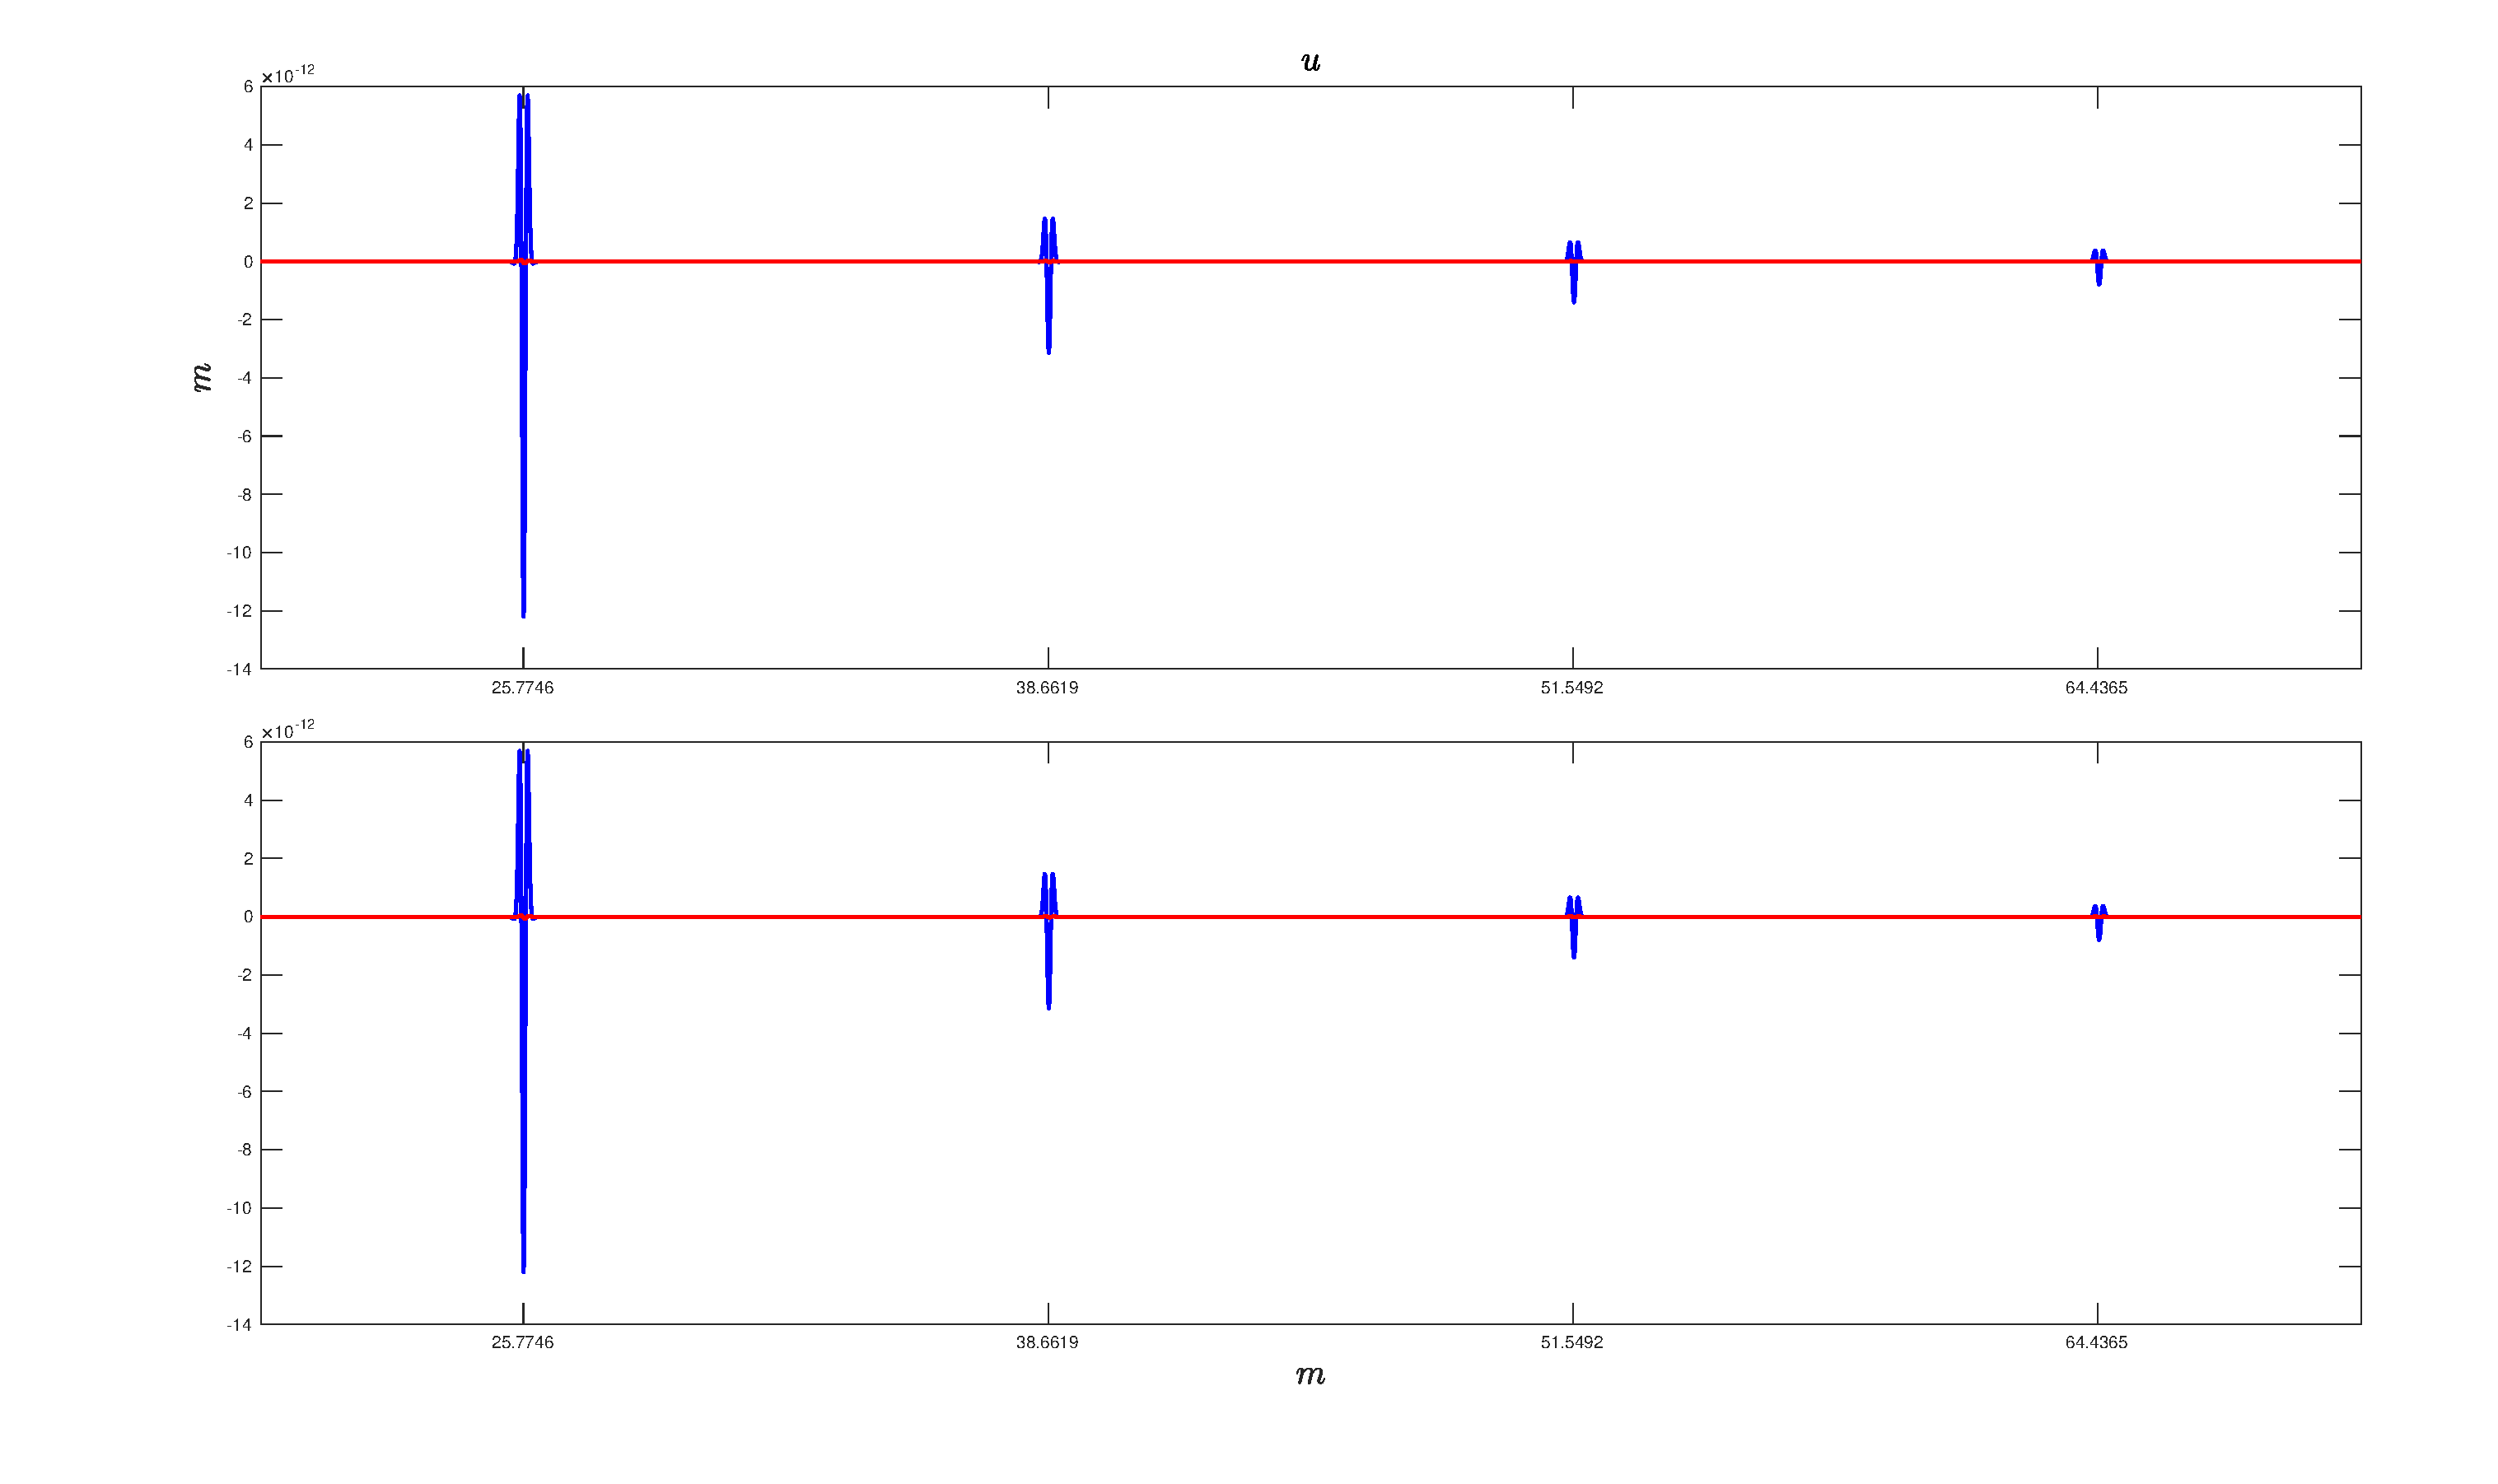
\includegraphics[scale=.5]{u_homo_F}
\caption{\textit{Tra\c{c}o s\'ismico de onda mec\^anica para sistema totalmente acoplado em cima e parcialmente acoplado embaixo, para pequenas dist\^ancias fonte/receptor.}}
\label{fig.mech_homo_low_dep}
\end{figure}
\end{landscape}

\begin{landscape}
\begin{figure}
\centering
\includegraphics[scale=1.05]{u_homo_large_depth}
\caption{\textit{Tra\c{c}o s\'ismico de onda mec\^anica para sistema totalmente acoplado em cima e parcialmente acoplado embaixo, para grandes dist\^ancias fonte/receptor.}}
\end{figure}
\label{fig.mag_homo_low_dep}
\end{landscape}

\begin{landscape}
\begin{figure}
\centering
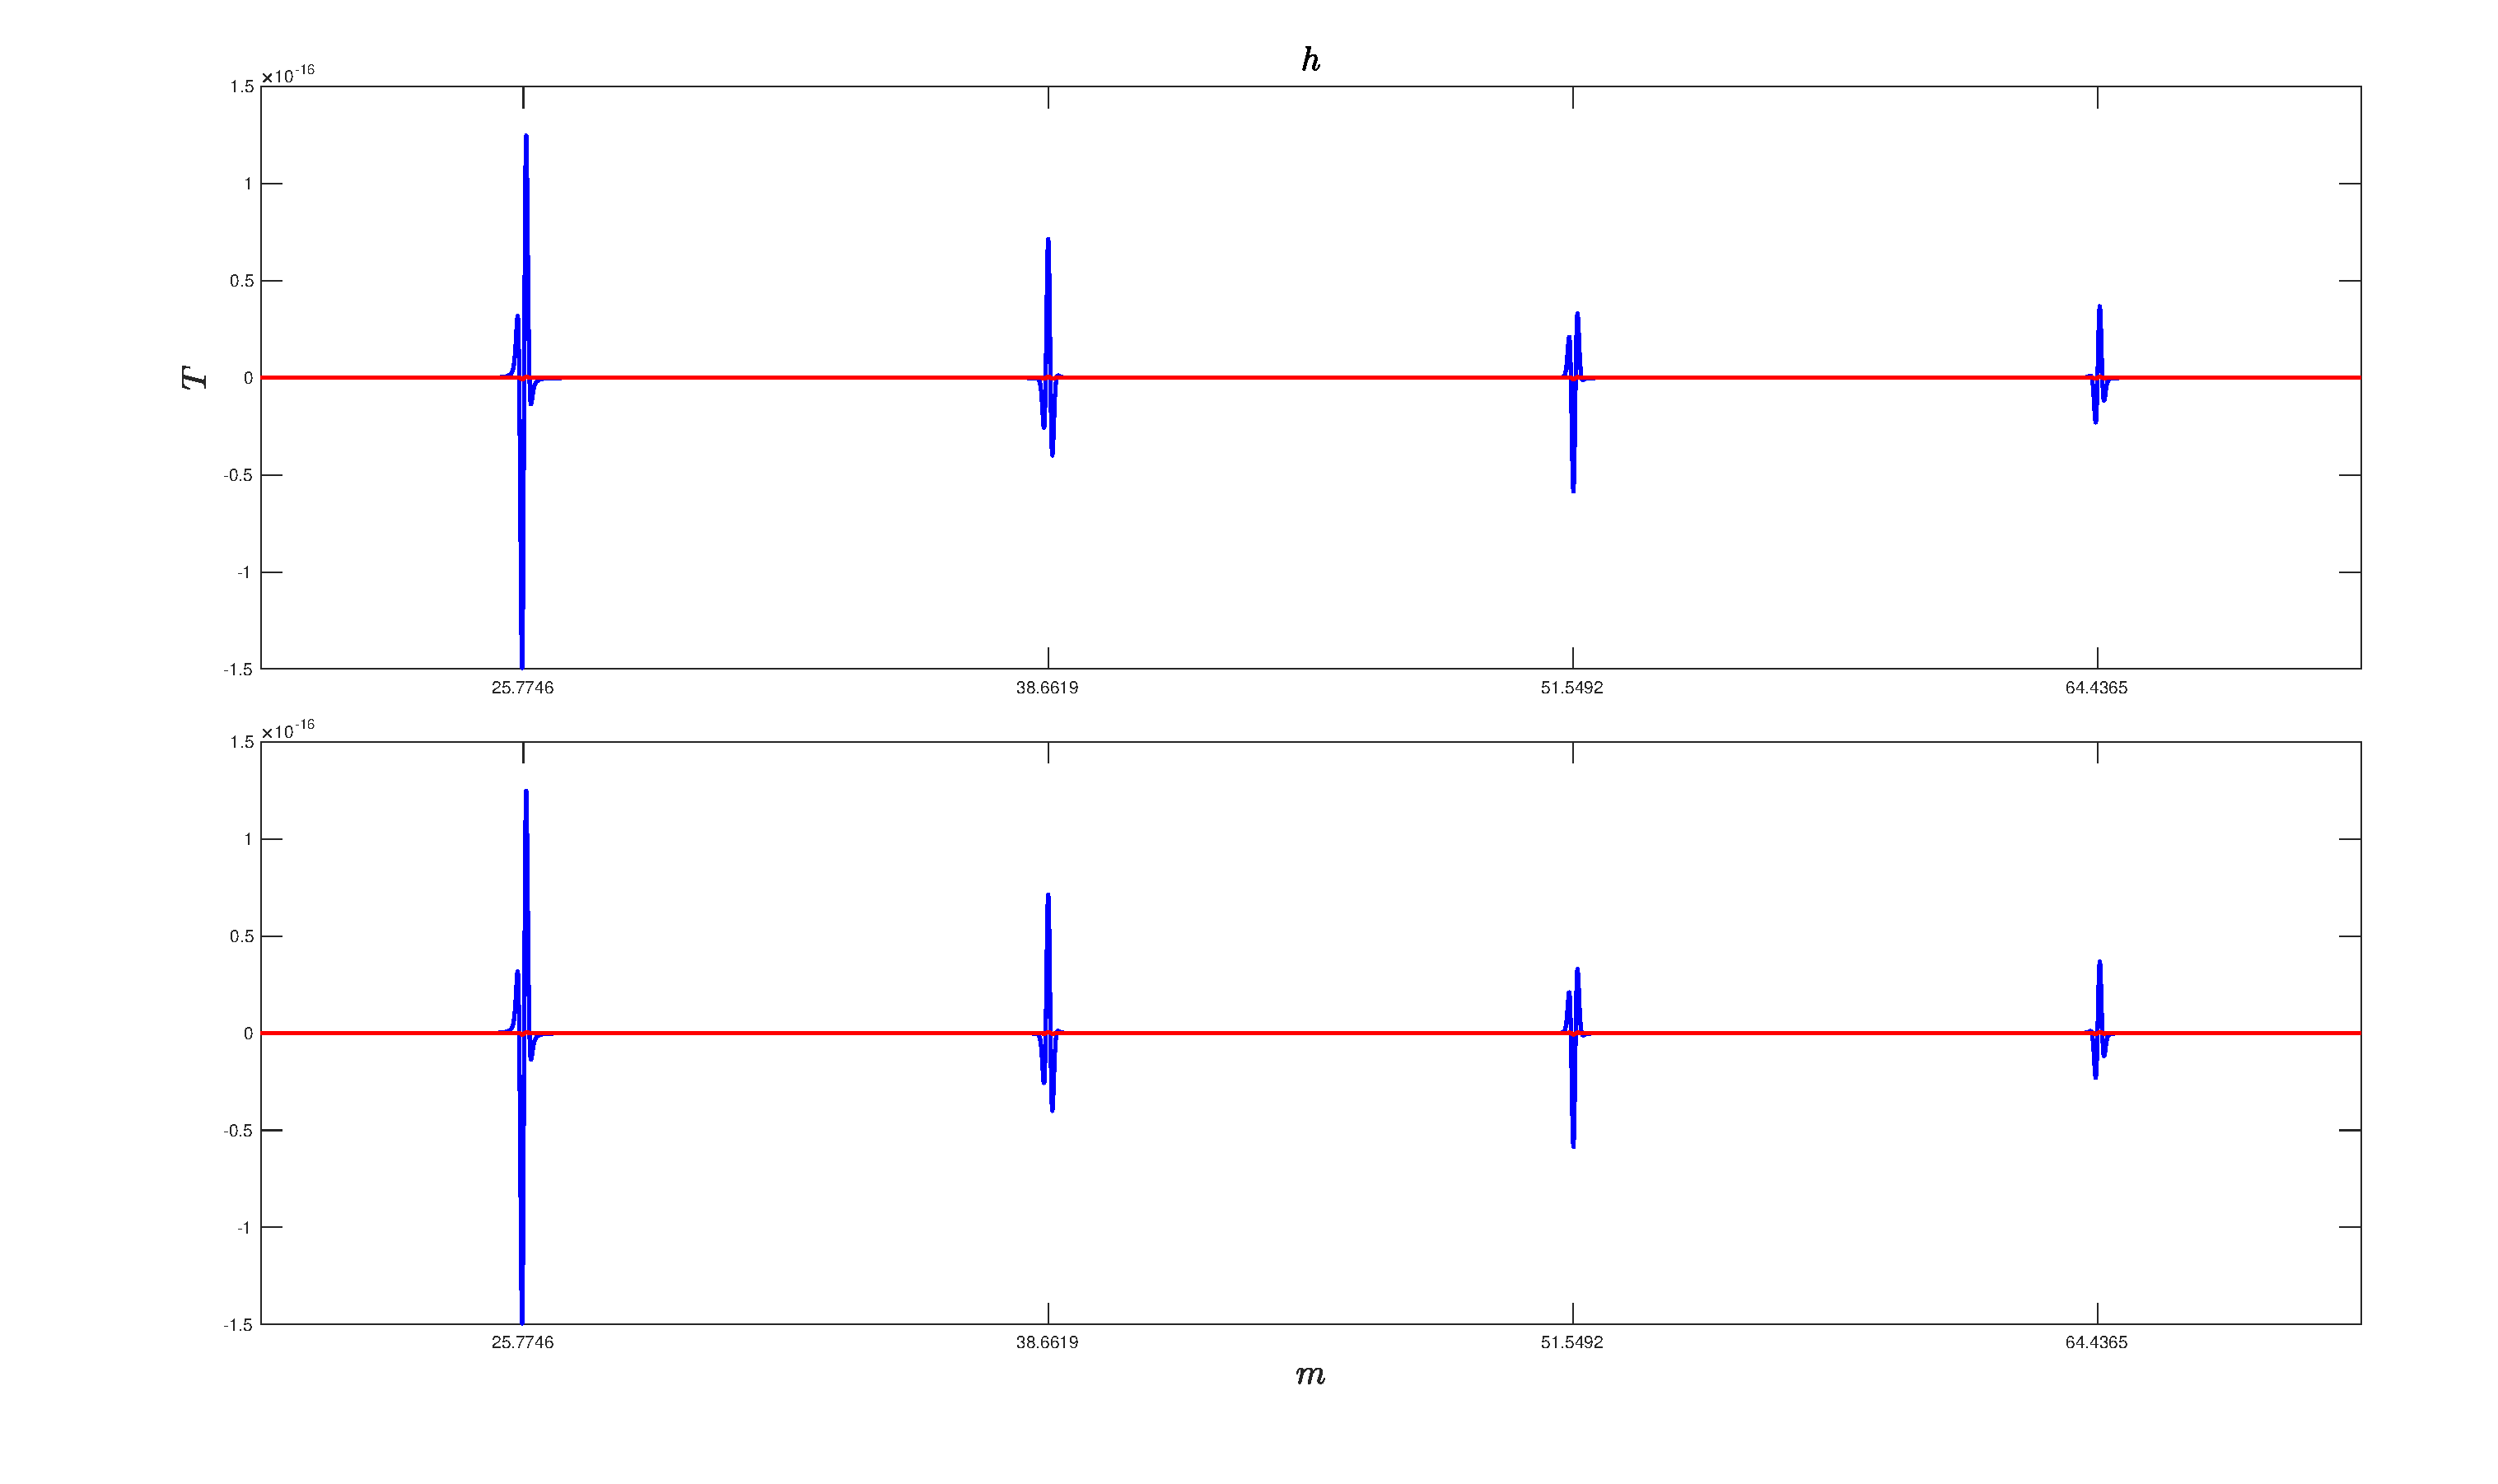
\includegraphics[scale=.5]{h_homo_F}
\caption{\textit{Tra\c{c}o s\'ismico do campo magn\'etico para sistema totalmente acoplado em cima e parcialmente acoplado embaixo, para pequenas dist\^ancias fonte/receptor.}}
\label{fig.mech_homo_high_dep}
\end{figure}
\end{landscape}

\begin{landscape}
\begin{figure}
\centering
\includegraphics[scale=1.05]{h_homo_large_depth}
\caption{\textit{Tra\c{c}o s\'ismico do campo magn\'etico para sistema totalmente acoplado em cima e parcialmente acoplado embaixo, para grandes dist\^ancias fonte/receptor.}}
\label{fig.mag_homo_high_dep}
\end{figure}
\end{landscape}

\section{Ondas em Meio Estratificado se Propagando em uma Dimens\~ao}\label{sec.prop_strat_1D}

\subsection{Acoplamento Total}\label{sec.1D_four_fully}

Partindo das EDO's (\ref{eq.edo_2}), (\ref{eq.edo_3}), (\ref{eq.edo_7}) e (\ref{eq.edo_10}), vamos incluir a for\c{c}a de Lorentz dada pela equa\c{c}\~ao TAL na equa\c{c}\~ao (\ref{eq.edo_10}), para trabalharmos em um modelo com acoplamento total entre campos mec\^anicos e eletromagn\'eticos. Assim, temos o seguinte sistema
\begin{align*}
\frac{\partial\,E}{\partial\,z}&=-i\,\omega\,\mu_0\,h\\\\
\frac{\partial\,h}{\partial\,z}&=\sigma\,E-i\,\omega\,\sigma\,\mu_0h^0u\\\\
\frac{\partial\,u}{\partial\,z}&=\frac{1}{\lambda+2\,G}\,\tau\\\\
\frac{\partial\,\tau}{\partial\,z}&=-\omega^2\,\rho\,u+\mu_0h^0\frac{\partial\,h}{\partial\,z}-F.
\end{align*}
Seguindo o algoritmo em formato matricial preconizado por \cite{ursin-1983}, temos
\begin{equation}\label{eq.four_f_full_coupled_1D_model}
\frac{\partial}{\partial\,z}\begin{pmatrix}
h\\
\tau\\
E\\
u
\end{pmatrix}
=
-i\,\omega\begin{pmatrix}
0&0&\frac{-\sigma}{i\,\omega}&\sigma\,\mu_0h^0\\
0&0&\frac{-\sigma\,\mu_0h^0}{i\,\omega}&\sigma\,\mu_0^2(h^0)^2-i\,\omega\rho\\
\mu_0&0&0&0\\
0&\frac{-1}{i\,\omega\,(\lambda+2\,G)} &0&0
\end{pmatrix}
\begin{pmatrix}
h\\
\tau\\
E\\
u
\end{pmatrix}
+
\begin{pmatrix}
0\\
-F\\
0\\
0
\end{pmatrix}.
\end{equation}
\begin{equation*}
M_1M_2=\begin{pmatrix}
\frac{\sigma\,\mu_0}{-i\,\omega}&\frac{-\sigma\,\mu_0h^0}{i\,\omega\,(\lambda+2\,G)}\\\\
\frac{\sigma\,\mu_0^2h^0}{-i\,\omega}&\frac{i\,\omega\rho-\sigma\,\mu_0^2(h^0)^2}{i\,\omega\,(\lambda+2\,G)}
\end{pmatrix}
=\begin{pmatrix}
m_{11}&m_{12}\\
m_{21}&m_{22}
\end{pmatrix}.
\end{equation*}
Sendo $q^2_{1,2}$ os autovalores para a matriz $M_1M_2$, temos que os autovetores s\~ao dados por
\begin{equation*}
\mathbf{a}_1=\begin{pmatrix}
a_1\\\\
\frac{q_1^2-m_{11}}{m_{12}}\,a_1
\end{pmatrix}\qquad\text{e}\qquad
\mathbf{a}_2=\begin{pmatrix}
\frac{m_{12}}{q_2^2-m_{11}}\,a_2\\\\
a_2
\end{pmatrix},
\end{equation*}
onde
\begin{equation*}
a_1=\sqrt{\frac{q_1}{\mu_0-\frac{(q_1^2-m_{11})^2}{i\,\omega\,m_{12}^2(\lambda+2\,G)}}}\qquad\text{e}\qquad 
a_2=\sqrt{\frac{q_2}{\frac{m_{12}^2\mu_0}{(q_2^2-m_{11})^2}-\frac{1}{i\,\omega\,(\lambda+2\,G)}}}.
\end{equation*}
Os autovalores para a matriz $M_2M_1$ tamb\'em s\~ao dados por $q_{1,2}^2$, e os autovetores s\~ao
\begin{equation*}
\mathbf{b}_1=\frac{1}{q_1}\begin{pmatrix}
\mu_0a_1\\\\
\frac{q_1^2-m_{11}}{-i\,\omega\,m_{12}(\lambda+2\,G)}\,a_1
\end{pmatrix}\qquad\text{e}\qquad
\mathbf{b}_2=\frac{1}{q_2}\begin{pmatrix}
\frac{\mu_0m_{12}}{q_2^2-m_{11}}\,a_2\\\\
\frac{1}{-i\,\omega\,(\lambda+2\,G)}a_2
\end{pmatrix}.
\end{equation*}
Vamos utilizar uma fonte n\~ao causal que simula a aplica\c{c}\~ao de uma for\c{c}a vertical dada por
\begin{equation*}
F=\delta(z-z_0)\,rck(\omega),
\end{equation*}
onde $\delta$ de \textit{Dirac} \'e a fun\c{c}\~ao dada pela subse\c{c}\~ao (\ref{sec.dirac}) e $rck(\omega)$ \'e o pulso de \textit{Ricker} no dom\'inio da frequ\^encia angular. Seguindo a subse\c{c}\~ao \ref{sec.presenca_fonte}, vamos substituir $F$ na fonte $\mathbf{S}$ e usar a rela\c{c}\~ao
\begin{equation*}
\mathbf{S}=\delta(z-z_0)\,\begin{pmatrix}
\mathbf{S_A}\\
\mathbf{S_B}
\end{pmatrix},
\end{equation*}
para obtermos
\begin{equation*}
\mathbf{S_A}=\begin{pmatrix}
0\\
rck
\end{pmatrix}\qquad\text{e}\qquad\mathbf{S_B}=\begin{pmatrix}
0\\
0
\end{pmatrix}.
\end{equation*}
As condi\c{c}\~oes de contorno s\~ao inseridas usando as matrizes $G_A$ e $G_B$, conforme a subse\c{c}\~ao \ref{sec.cond_contorno},
\begin{equation*}
\mathbf{\Phi}=\begin{pmatrix}
G_A\\
G_B
\end{pmatrix}\mathbf{\Phi}_g,
\end{equation*}
onde
\begin{equation*}
G_A=\begin{pmatrix}
\frac{q_0}{\mu_0}&0\\
0&0
\end{pmatrix},\qquad G_B=\begin{pmatrix}
1&0\\
0&1
\end{pmatrix}\qquad\text{e}\qquad\mathbf{\Phi}_g=\begin{pmatrix}
E\\
u
\end{pmatrix}.
\end{equation*}
Assim, podemos obter numericamente as solu\c{c}\~oes para o sistema (\ref{eq.four_f_full_coupled_1D_model}), em que duas delas t\^em seus gr\'aficos nas figuras (\ref {fig.four_fully_1D_u}) e (\ref{fig.four_fully_1D_h}), onde podemos observar, respectivamente, o campo mec\^anico e o campo magn\'etico de ondas que se propagam em camadas estratigr\'aficas. Para esta simula\c{c}\~ao estamos considerando uma geometria estratigr\'afica com duas camadas onde a camada 1 tem a superf\'icie livre de contato com o ar e tem $1000\,m$ de profundidade. A camada 1, que \'e onde ocorre a propaga\c{c}\~ao, forma uma interface de contato com a camada 2 a qual possui profundidade infinita, e as caracter\'sticas dessas camadas est\~ao na tabela (\ref{tab.dados_propagacao}). Tanto na figura  (\ref {fig.four_fully_1D_u}) como na figura (\ref{fig.four_fully_1D_h}) podemos visualizar nitidamente tr\^es eventos para a onda mec\^anica e eletromagn\'etica, respectivamente. Nesses dois gr\'aficos temos a chegada de uma onda direta no tempo zero (simulando com fonte n\~ao causal e receptor na mesma posi\c{c}\~ao), seguida de uma reflex\~ao na interface entre a primeira e segunda camadas, e por \'ultimo uma m\'ultipla da referida reflex\~ao. A interface est\'a a 1000 $m$ de profundidade em rela\c{c}\~ao \`a superficie livre onde est\'a a fonte, e observamos que a m\'ultipla tem o dobro do tempo de chegada em rela\c{c}\~ao \`a sua correspondente reflex\~ao, para ambas as ondas. Como estamos trabalhando com modelo de acoplamento entre as ondas, o tempo de chegada da reflex\~ao da onda mec\^anica \'e bastante pr\'oximo do tempo da onda eletromagn\'etica, e o tempo de chegada tamb\'em \'e similar entre as m\'ultiplas dessas duas ondas.

\begin{figure}
\centering
\includegraphics[scale=.9]{four_fully_1D_u}\\
\caption{\textit{Campo mec\^anico em acoplamento total, com fonte e receptor na superf\'icie e interface a 1000 $m$. Observamos a onda direta, seguida da reflex\~ao e depois uma m\'ultipla.}}
\label{fig.four_fully_1D_u}
\end{figure}


\begin{figure}
\centering
\includegraphics[scale=.825]{four_fully_1D_h}\\
\caption{\textit{Campo magn\'etico em acoplamento total, com fonte e receptor na superf\'icie e interface a 1000 $m$. Observamos a onda direta, seguida da reflex\~ao e depois uma m\'ultipla.}}
\label{fig.four_fully_1D_h}
\end{figure}


\subsection{Acoplamento Parcial}
Para tratarmos do acoplamento parcial, vamos desconsiderar a influ\^encia que os campos eletromagn\'eticos exercem sobre os campos mec\^anicos, ou seja, o modelo dado pelas equa\c{c}\~oes \ref{eq.four_f_full_coupled_1D_model} \'e reescrito como
\begin{equation*}
\frac{\partial}{\partial\,z}\begin{pmatrix}
h\\
\tau\\
E\\
u
\end{pmatrix}
=
-i\,\omega\begin{pmatrix}
0&0&\frac{-\sigma}{i\,\omega}&\sigma\,\mu_0h^0\\
0&0&0&\sigma\,\mu_0^2(h^0)^2-i\,\omega\rho\\
\mu_0&0&0&0\\
0&\frac{-1}{i\,\omega\,(\lambda+2\,G)} &0&0
\end{pmatrix}
\begin{pmatrix}
h\\
\tau\\
E\\
u
\end{pmatrix}
+
\begin{pmatrix}
0\\
-F\\
0\\
0
\end{pmatrix},
\end{equation*}
e a matriz $M_1M_2$ passa a ser dada por
\begin{equation*}
M_1M_2=\begin{pmatrix}
\frac{\sigma\,\mu_0}{-i\,\omega}&\frac{-\sigma\,\mu_0h^0}{i\,\omega\,(\lambda+2\,G)}\\\\
0&\frac{i\,\omega\rho-\sigma\,\mu_0^2(h^0)^2}{i\,\omega\,(\lambda+2\,G)}
\end{pmatrix}
=\begin{pmatrix}
m_{11}&m_{12}\\
m_{21}&m_{22}
\end{pmatrix}.
\end{equation*}
Os autovalores e autovetores, fonte e condi\c{c}\~oes de contorno para esse novo modelo podem ser calculados usando as mesmas f\'ormulas da subse\c{c}\~ao \ref{sec.1D_four_fully}, bastando tomar $m_{21}=0$ para determinarmos os autovalores. As solu\c{c}\~oes podem ser observadas nas figuras (\ref{fig.four_partially_1D_mech}) e (\ref{fig.four_partially_1D_eletro}).

\begin{figure}
\centering
\includegraphics[scale=.71]{four_partially_1D_u}\\
\caption{\textit{Podemos observar a chegada da onda direta seguida de uma reflex\~ao e uma m\'ultipla de uma onda mec\^anica, num sistema parcialmente acoplado.}}
\label{fig.four_partially_1D_mech}
\end{figure}

\begin{figure}
\centering
\includegraphics[scale=.85]{four_partially_1D_h}\\
\caption{\textit{Onda direta seguida de uma reflex\~ao e uma m\'ultipla (de amplitude bem pequena) de uma onda eletromagn\'etica, num sistema parcialmente acoplado.}}
\label{fig.four_partially_1D_eletro}
\end{figure}

Comparando os campos mec\^anicos do modelo de acoplamento total na figura (\ref{fig.four_fully_1D_u}) com o modelo de acoplamento parcial na figura (\ref{fig.four_partially_1D_mech}), observamos que n\~ao houve altera\c{c}\~ao significativa na propaga\c{c}\~ao dessas ondas quando mudamos o modelo. Os tempos de chegada e as amplitudes das ondas diretas, das reflex\~oes na primeira interface e das respectivas m\'ultiplas, permanecem aproximadamente iguais. Quaisquer discrep\^ancias entre os gr\'aficos podem estar relacionadas \`a estabilidade num\'erica, j\'a que para o caso parcialmente acoplado estamos computando uma quantidade menor de dados e, consequentemente, seu gr\'afico pode apresentar menos ru\'ido e sinais de instabilidade. 

Vamos mudar algumas caracter\'isticas da segunda camada para alterarmos a rela\c{c}\~ao de imped\^ancia e o coeficiente de reflex\~ao entre a primeira e segunda camadas para uma melhor visualiza\c{c}\~ao dos eventos. Em rela\c{c}\~ao \`a tabela (\ref{tab.dados_propagacao}), alteramos a segunda camada para $\rho=3000\,\frac{kg}{m^3}$ e $\sigma=1\,S/m$ (uma caracter\'istica mec\^anica e uma eletromagn\'etica), e com isso conseguimos uma melhor visualiza\c{c}\~ao da reflex\~ao e das m\'ultiplas na figura (\ref{fig.four_partially_1D_mech_hi_ampl}) para onda mec\^anica e na figura (\ref{fig.four_partially_1D_electro_hi_ampl}) para onda eletromagn\'etica. Comparando as figuras (\ref{fig.four_partially_1D_mech}) e (\ref{fig.four_partially_1D_mech_hi_ampl}), al\'em de termos  um aumento nas amplitudes da reflex\~ao e das m\'ultiplas, aumentamos tamb\'em a quantidade de m\'ultiplas vis\'iveis. Note ainda que o tempo de chegada da reflex\~ao e das m\'ultiplas n\~ao foram alterados, pois s\'o mudamos as caracter\'isticas da segunda camada e a onda mec\^anica est\'a se propagando na primiera. Essa mesma an\'alise pode ser aplicada \`a onda eletromagn\'etica comparando as figuras (\ref{fig.four_partially_1D_eletro}) e (\ref{fig.four_partially_1D_electro_hi_ampl}).

\begin{figure}
\centering
\includegraphics[scale=.36]{four_partially_1D_high_ampl_u}\\
\caption{\textit{Podemos observar a chegada da onda direta seguida de uma reflex\~ao e de tr\^es m\'ultiplas da onda mec\^anica.}}
\label{fig.four_partially_1D_mech_hi_ampl}
\end{figure}


\begin{figure}
\centering
\includegraphics[scale=.94]{four_partially_1D_high_ampl_h}\\
\caption{\textit{Podemos observar a chegada da onda direta seguida de uma reflex\~ao e de tr\^es m\'ultiplas da onda eletromagn\'etica.}}
\label{fig.four_partially_1D_electro_hi_ampl}
\end{figure}

At\'e aqui temos simulado propaga\c{c}\~ao com o receptor na superf\'icie, teoricamente junto com a fonte, numa camada de 1000 $m$ de espessura. Mas podemos simular com o receptor em profundidades variadas, e na figura (\ref{fig.four_partially_1D_mech_hi_ampl_250}) vemos uma simula\c{c}\~ao para onda mec\^anica com o receptor a $250\,m$ de profundidade, de onde extra\'imos algumas observa\c{c}\~oes.

\begin{itemize}
\item A chegada da onda direta (evento 1) n\~ao ocorre mais exatamente no tempo zero (considerando fonte n\~ao causal) como acontece com o receptor na superf\'icie, pois a onda teve que descer por 250 $m$ at\'e que atingisse o receptor.
\item A onda refletida na interface entre as camadas (evento 2) chega com tempo um pouco menor que a reflex\~ao do modelo anterior comparando com a figura (\ref{fig.four_partially_1D_mech_hi_ampl}), por exemplo. De fato, para produzir a reflex\~ao do modelo com receptor na superf\'icie, a onda se propagou por $2000\,m$ ida e volta, e aqui a onda se propagou por $1750\,m$.
\item Existe uma grande diferen\c{c}a de amplitude entre a onda refletida e a onda direta, j\'a que al\'em da perda de energia para o meio durante a propaga\c{c}\~ao houve tamb\'em a perda de energia na interface entre as camadas por conta da onda transmitida para a segunda camada.
\item A onda refletida na interface produziu o evento 2, continuou subindo, foi refletida na superf\'icie livre e desceu novamente produzindo o evento 3.
\item Entre os eventos 2 e 3 a onda se propagou por apenas $500\,m$, por isso o evento 3 ocorre rapidamente ap\'os o evento 2.
\item A reflex\~ao na superf\'icie livre \'e praticamente total e n\~ao h\'a onda transmitida para a camada de ar. Assim, h\'a pouca diminui\c{c}\~ao da amplitude do evento 3 em rela\c{c}\~ao ao evento 2, a qual \'e devida somente a perda de energia para o meio durante a propaga\c{c}\~ao.
\item Os eventos 4 e 5 s\~ao m\'ultiplas dos eventos 2 e 3. A grande diminui\c{c}\~ao da amplitude do evento 4 em rela\c{c}\~ao ao evento 3 e a pouca diminui\c{c}\~ao do evento 5 em rela\c{c}\~ao ao 4 ocorrem pelas mesmas raz\~oes dos itens anteriores.
\item Podemos visualizar a ocorr\^encia de mais m\'ultiplas ap\'os o evento 5.
\end{itemize}

\begin{figure}
\centering
\includegraphics[scale=.775]{four_partially_1D_high_ampl_250_u}\\
\caption{\textit{Camada com 1000 $m$, fonte na superf\'icie e o receptor a 250 $m$ de profundidade.}}
\label{fig.four_partially_1D_mech_hi_ampl_250}
\end{figure}

\begin{figure}
\centering
\includegraphics[scale=.87]{four_partially_1D_high_ampl_750_u}\\
\caption{\textit{Camada com 1000 $m$, fonte na superf\'icie e o receptor a 750 $m$ de profundidade.}}
\label{fig.four_partially_1D_mech_hi_ampl_750}
\end{figure}

Na figura (\ref{fig.four_partially_1D_mech_hi_ampl_750}) podemos observar uma simula\c{c}\~ao de propaga\c{c}\~ao de onda mec\^anica numa camada com espessura de 1000 $m$, fonte na superf\'icie e com receptor a 750 $m$ de profundidade, de onde podemos retirar mais algumas observa\c{c}\~oes.

\begin{itemize}
\item O tempo de chegada da onda direta (evento 1) \'e maior que nos dois casos anteriores com receptor na superf\'icie e receptor a $250\,m$ de profundidade. 
\item  Existe pouca diferen\c{c}a de tempo entre a onda direta e a onda refletida na interface (evento 2), pois o receptor se encontra pr\'oximo \`a interface e entre esses eventos a onda se propagou por apenas $500\,m$.
\item A onda refletida na interface (evento 2) atinge o receptor com amplitude bem menor que da onda direta (evento 1), pois h\'a perda de energia da onda transmitida para a segunda camada.
\item O tempo, desde o acionamento da fonte, com que a onda refletida na interface (evento 2) atinge o receptor \'e menor que nos dois casos anteriores (figuras (\ref{fig.four_partially_1D_mech_hi_ampl}) e (\ref{fig.four_partially_1D_mech_hi_ampl_250})), pois aqui essa onda se propagou por uma dist\^ancia menor, $1250\,m$.
\item Ap\'os produzir o evento 2, a onda refletida na interface continua subindo, \'e refletida na superf\'icie livre e desce novamente para produzir o evento 3, completando um ciclo. Ou seja, o evento 3 \'e uma m\'ultipla do evento 1.
\item A diminui\c{c}\~ao de amplitude do evento 3 em rela\c{c}\~ao ao evento 2 n\~ao \'e muito grande, pois a onda sofre reflex\~ao total na superf\'icie livre, e a diminui\c{c}\~ao de amplitude detectada deve-se basicamente a perda de energia para o meio durante a propaga\c{c}\~ao.
\item O evento 4 (m\'ultipla do evento 2) \'e a segunda reflex\~ao na interface e atinge o receptor, comparando com o evento 3, num tempo curto e com amplitude bastante reduzida por conta da energia transmitida para segunda camada.
\item Podemos visualizar mais m\'ultiplas ap\'os o evento 4.
\end{itemize}

\section{Ondas em Meio Estratificado se Propagando em tr\^es Dimens\~oes}
Nesse modelo onde consideramos a propaga\c{c}\~ao em tr\^es dimens\~oes podemos estudar tamb\'em o comportamento da onda transversal, ou onda $S$. A geometria estratigr\'afica \'e composta por tr\^es camadas: a camada 1 com $1000\,m$ de profundidade e superf\'icie livre de contato com o ar, a camada 2 com $500\,m$ de profundidade, interface superior de contato com a camada 1 e interface inferiror de contato com a camada 3, onde a camada 3 possui profundidade infinita. Analisamos somente as ondas que se propagam nas camadas 1 e 2, e as caracter\'isticas das tr\^es camadas est\~ao na tabela (\ref{tab.dados_propagacao}). Assim, nas figuras (\ref{fig.v3}) e (\ref{fig.v3_750}) observamos tra\c{c}os s\'ismicos com v\'arias amplitudes que representam as chegadas de ondas $P$ ou $S$ refletidas na primeira ou segunda interfaces, bem como suas m\'ultiplas.

No cap\'itulo (\ref{sec.disp_aten_mag_elastico}), constatamos que a influ\^encia de campos eletromagn\'eticos em campos mec\^anicos \'e desprez\'ivel em rela\c{c}\~ao a an\'alise de dispers\~ao e atenua\c{c}\~ao, em simula\c{c}\~oes com v\'arios modelos. De acordo com as subse\c{c}\~oes (\ref{sec.prop_homo_1D}) e (\ref{sec.prop_strat_1D}), constatamos ainda que a influ\^encia de campos eletromagn\'eticos em campos mec\^anicos tamb\'em \'e desprez\'ivel em modelos de propaga\c{c}\~ao em uma dimens\~ao tanto homog\^eneos como estratificados. Essas duas constata\c{c}\~oes sugerem que essa influ\^encia continue sendo desprez\'ivel para modelos de propaga\c{c}\~ao em tr\^es dimens\~oes, e isso se constitui numa nova hip\'otese simplificadora para nosso problema, j\'a que n\~ao \'e poss\'ivel ajustar nosso modelo ao formato preconizado por \cite{Ursin-1983}, nem mesmo com a adapta\c{c}\~ao do algoritmo usada nos casos anteriores. Assim, estudamos o caso de propaga\c{c}\~ao em tr\^es dimens\~oes usando apenas o modelo para sistemas parcialmente acoplados, onde analisamos o comportamento somente de campos mec\^anicos para em seguida observar quais influ\^encias esse comportamento mec\^anico provoca em campos eletromagn\'eticos.

\subsection{Modelo para Ondas Mec\^anicas}
Para tratar as ondas mec\^anicas sem influ\^encia dos campos eletromagn\'eticos usamos as equa\c{c}\~oes (\ref{eq.edo_5}) at\'e (\ref{eq.edo_10}), as quais j\'a est\~ao no formato sem aplica\c{c}\~ao da for\c{c}a de \textit{Lorentz}. Para possibilitar a utiliza\c{c}\~ao do m\'etodo matricial dividimos as equa\c{c}\~oes em dois sistemas, onde $v=\dot{\tilde{u}}$ \'e a velocidade de deslocamento do meio.

\begin{empheq}[left=\empheqlbrace]{align}\nonumber
\frac{\partial\,v_3}{\partial\,z}&=-\frac{i\,\omega}{\lambda+2\,G}\,\tilde{\tau}_{33}-\frac{i\,\omega\,\gamma\,\lambda}{\lambda+2\,G}\,v_1\\\nonumber\\\nonumber
\frac{\partial\,\tilde{\tau}_{13}}{\partial\,z}&=-i\,\omega
\left(\rho-\frac{4\,\gamma^2G\,(\lambda+G)}{\lambda+2\,G}\right)\,v_1-\frac{i\,\omega\,\gamma\,\lambda}{\lambda+2\,G}\,\tilde{\tau}_{33}-\tilde{F}_1\\\label{eq.sys_mech_1}\\\nonumber
\frac{\partial\,\tilde{\tau}_{33}}{\partial\,z}&=\frac{\omega\,\rho}{i}\,v_3-i\,\omega\,\gamma\,\tilde{\tau}_{13}-\tilde{F}_3\\\nonumber\\\nonumber
\frac{\partial\,v_1}{\partial\,z}&=-i\,\gamma\,\omega\,v_3-\frac{i\,\omega}{G}\,\tilde{\tau}_{13}
\end{empheq}

\begin{empheq}[left=\empheqlbrace]{align}\nonumber
\frac{\partial\,v_2}{\partial\,z}&=-\frac{i\,\omega}{G}\,\tilde{\tau}_{23}\\\label{eq.sys_mech_2}\\\nonumber
\frac{\partial\,\tilde{\tau}_{23}}{\partial\,z}&=\left[\frac{\omega\,\rho}{i}+\frac{i^2\gamma^2\omega\,G}{i}\right]\,v_2-\tilde{F}_2
\end{empheq}

Come\c{c}ando com o sistema (\ref{eq.sys_mech_1}), temos
\begin{equation*}
M_1^{(\ref{eq.sys_mech_1})}=\begin{pmatrix}
\frac{1}{\lambda+2\,G}&\frac{\gamma\,\lambda}{\lambda+2\,G}\\\\
\frac{\gamma\,\lambda}{\lambda+2\,G}\,&\,\rho-\frac{4\,\gamma^2G\,(\lambda+G)}{\lambda+2\,G}
\end{pmatrix}\,,\quad\quad
M_2^{(\ref{eq.sys_mech_1})}=\begin{pmatrix}
\rho&\gamma\\\\
\gamma&\frac{1}{G}
\end{pmatrix}\quad\text{e}\quad
\mathbf{S}^{(\ref{eq.sys_mech_1})}=\begin{pmatrix}
0\\-F_1\\-F_3\\0
\end{pmatrix},
\end{equation*}
e os autovetores s\~ao
\begin{equation*}
\mathbf{a}_1^{(\ref{eq.sys_mech_1})}=
\sqrt{\frac{q_1}{ \rho+2\,\gamma\,a_1+\frac{a_1^2}{G}}}
\begin{pmatrix}
1\\
a_1
\end{pmatrix}\quad\text{e}\quad
\mathbf{a}_2^{(\ref{eq.sys_mech_1})}=
\sqrt{\frac{q_2}{a_2^2\rho+2\,\gamma\,a_2+\frac{1}{G}}}
\begin{pmatrix}
a_2\\
1
\end{pmatrix}
\end{equation*}\\
\begin{equation*}
\mathbf{b}_1^{(\ref{eq.sys_mech_1})}=\frac{1}{q_1}M_2^{(\ref{eq.sys_mech_1})}\mathbf{a}_1^{(\ref{eq.sys_mech_1})}
\quad\text{e}\quad
\mathbf{b}_2^{(\ref{eq.sys_mech_1})}=\frac{1}{q_2}M_2^{(\ref{eq.sys_mech_1})}\mathbf{a}_2^{(\ref{eq.sys_mech_1})},
\end{equation*}
onde
\begin{equation*}
a_1=\frac{q_1^2- \frac{1}{\lambda+2\,G}  }{\frac{\gamma\,\lambda}{\lambda+2\,G}}\quad\text{e}\quad
a_2=\frac{\frac{\gamma\,\lambda}{\lambda+2\,G}}{q_2^2- \frac{1}{\lambda+2\,G}}.
\end{equation*}
Utilizamos como fonte a aplica\c{c}\~ao de uma for\c{c}a vertical que, no dom\'inio da frequ\^encia angular, \'e dada por
\begin{equation*}
\mathbf{F}=\begin{pmatrix}
0\\
0\\
rck(\omega)
\end{pmatrix}\delta(z-z_s),\quad\text{e como}\quad
\begin{pmatrix}
0\\
-F_1\\
-F_3\\
0
\end{pmatrix}
=-
\begin{pmatrix}
\mathbf{S}_A\\
\mathbf{S}_B
\end{pmatrix}\,\delta(z-z_s),
\end{equation*}
temos que
\begin{equation*}
\mathbf{S}_A^{(\ref{eq.sys_mech_1})}=\begin{pmatrix}
0\\
0
\end{pmatrix}\quad\text{e}\quad
\mathbf{S}_B^{(\ref{eq.sys_mech_1})}=\begin{pmatrix}
rck(\omega)\\
0
\end{pmatrix}.
\end{equation*}
Estabelecemos as condi\c{c}\~oes de contorno usando as encontradas em \cite{pride_94}, que s\~ao $\tau_{13}=\tau_{33}=0$, e a solu\c{c}\~ao imediatamente abaixo da superf\'icie \'e
\begin{equation*}
\Phi(0^+)^{(\ref{eq.sys_mech_1})}=\begin{pmatrix}
v_3\\
0\\
0\\
v_1
\end{pmatrix},\quad\text{e tomando}\quad
\Phi_g^{(\ref{eq.sys_mech_1})}=\begin{pmatrix}
v_3\\
v_1
\end{pmatrix},
\end{equation*}
temos que
\begin{equation*}
G_A^{(\ref{eq.sys_mech_1})}=\begin{pmatrix}
1&0\\
0&0
\end{pmatrix}\quad\text{e}\quad
G_B^{(\ref{eq.sys_mech_1})}=\begin{pmatrix}
0&0\\
0&1
\end{pmatrix}.
\end{equation*}

Para o sistema (\ref{eq.sys_mech_2}), temos 
\begin{equation*}
M_1^{(\ref{eq.sys_mech_2})}=\begin{pmatrix}
\frac{1}{G}
\end{pmatrix}\,,\quad\quad
M_2^{(\ref{eq.sys_mech_2})}=\begin{pmatrix}
\rho-G\,\gamma^2
\end{pmatrix}\quad\text{e}\quad
\mathbf{S}^{(\ref{eq.sys_mech_2})}=\begin{pmatrix}
0\\-F_2
\end{pmatrix},
\end{equation*}
e os autovetores s\~ao
\begin{equation*}
\mathbf{a}^{(\ref{eq.sys_mech_2})}=
\sqrt{\frac{q}{\rho-G\,\gamma^2}}
\quad\text{e}\quad
\mathbf{b}^{(\ref{eq.sys_mech_2})}=
\sqrt{\frac{\rho-G\,\gamma^2}{q}}.
\end{equation*}
Incluindo a fonte no m\'etodo matricial, temos
\begin{equation*}
\begin{pmatrix}
0\\
-F_2
\end{pmatrix}
=-
\begin{pmatrix}
S_A\\
S_B
\end{pmatrix}\,\delta(z-z_s)\quad\text{e, portanto,}\quad
\mathbf{S}_A^{(\ref{eq.sys_mech_2})}=\mathbf{S}_B^{(\ref{eq.sys_mech_2})}=0.
\end{equation*}
Ou seja, o tipo de fonte que estamos usando n\~ao produz onda para o sistema (\ref{eq.sys_mech_2}), pois esse sistema \'e respons\'avel por ondas $SH$, como podemos ver em \cite{pride_94}.

Na figura (\ref{fig.v3}), observamos o tra\c{c}o s\'ismico de uma onda mec\^anica obtido em simula\c{c}\~ao com o sistema (\ref{eq.sys_mech_1}), usando fonte e receptor na mesma posi\c{c}\~ao na superf\'icie.
\begin{figure}
\centering
\includegraphics[scale=.775]{v3}\\
\caption{\textit{Modelo tridimensional, primeira camada com 1000 $m$, segunda camada com 500 $m$, fonte e o receptor na superf\'icie.}}
\label{fig.v3}
\end{figure}
Vamos listar algumas observa\c{c}\~oes sobre essa propaga\c{c}\~ao:
\begin{itemize}
\item A ocorr\^encia do evento 1 no tempo zero mostra que este representa a onda direta, j\'a que receptor e fonte est\~ao juntos. Note que a amplitude da onda direta est\'a relativamente pequena.
\item O evento 2 ocorre no tempo necess\'ario para a onda $P$ realizar a propaga\c{c}\~ao de ida e volta entre a superf\'icie e a primeira interface, mostrando que este evento representa a reflex\~ao na primeira interface. 
\item O evento 3 ocorre no tempo necess\'ario para que a onda $S$ se propague ida e volta da superf\'icie at\'e a primeira interface, portanto \'e a reflex\~ao da onda $S$ na primeira interface. De fato, a amplitude do evento 3 \'e maior que do evento 2, comportamento comum entre ondas $P$ e $S$ como podemos observar em v\'arios sism\'ografos.
\item O tempo de chegada do evento 4 coincide com o tempo necess\'ario para onda longitudinal ser refletida na segunda interface.
\item O evento 5 tem o dobro do tempo de chegada e menor amplitude que o evento 2, mostrando que o mesmo \'e uma m\'ultipla da onda longitudinal refletida na primeira interface.
\item O evento 4 \'e de uma onda $P$ que viajou por $3000\,m$ e o evento 5 de uma onda $P$ que viajou por $4000\,m$, mas o evento 4 tem amplitude menor que do evento 5. Isso acontece porque o evento 4 passou por tr\^es processos (duas transmiss\~oes e uma reflex\~ao) de perda de energia em interfaces, enquanto o evento 5 passou por dois processos. 
\item O evento 6 tem o tempo de chegada compat\'ivel com o tempo necess\'ario para reflex\~ao de uma onda transversal na segunda interface. Note que o evento 6 tem amplitude e tempo de chegada maiores que do evento 4.
\item O evento 7 tem o dobro do tempo de chegada do evento 3, ou seja, \'e uma m\'ultipla da onda transversal refletida na primeira interface.
\item O evento 8 tem tr\^es vezes o tempo de chegada do evento 2, ou seja, \'e a segunda m\'ultipla da reflex\~ao da onda $P$ na primeira interface.
\end{itemize}

\begin{figure}
\centering
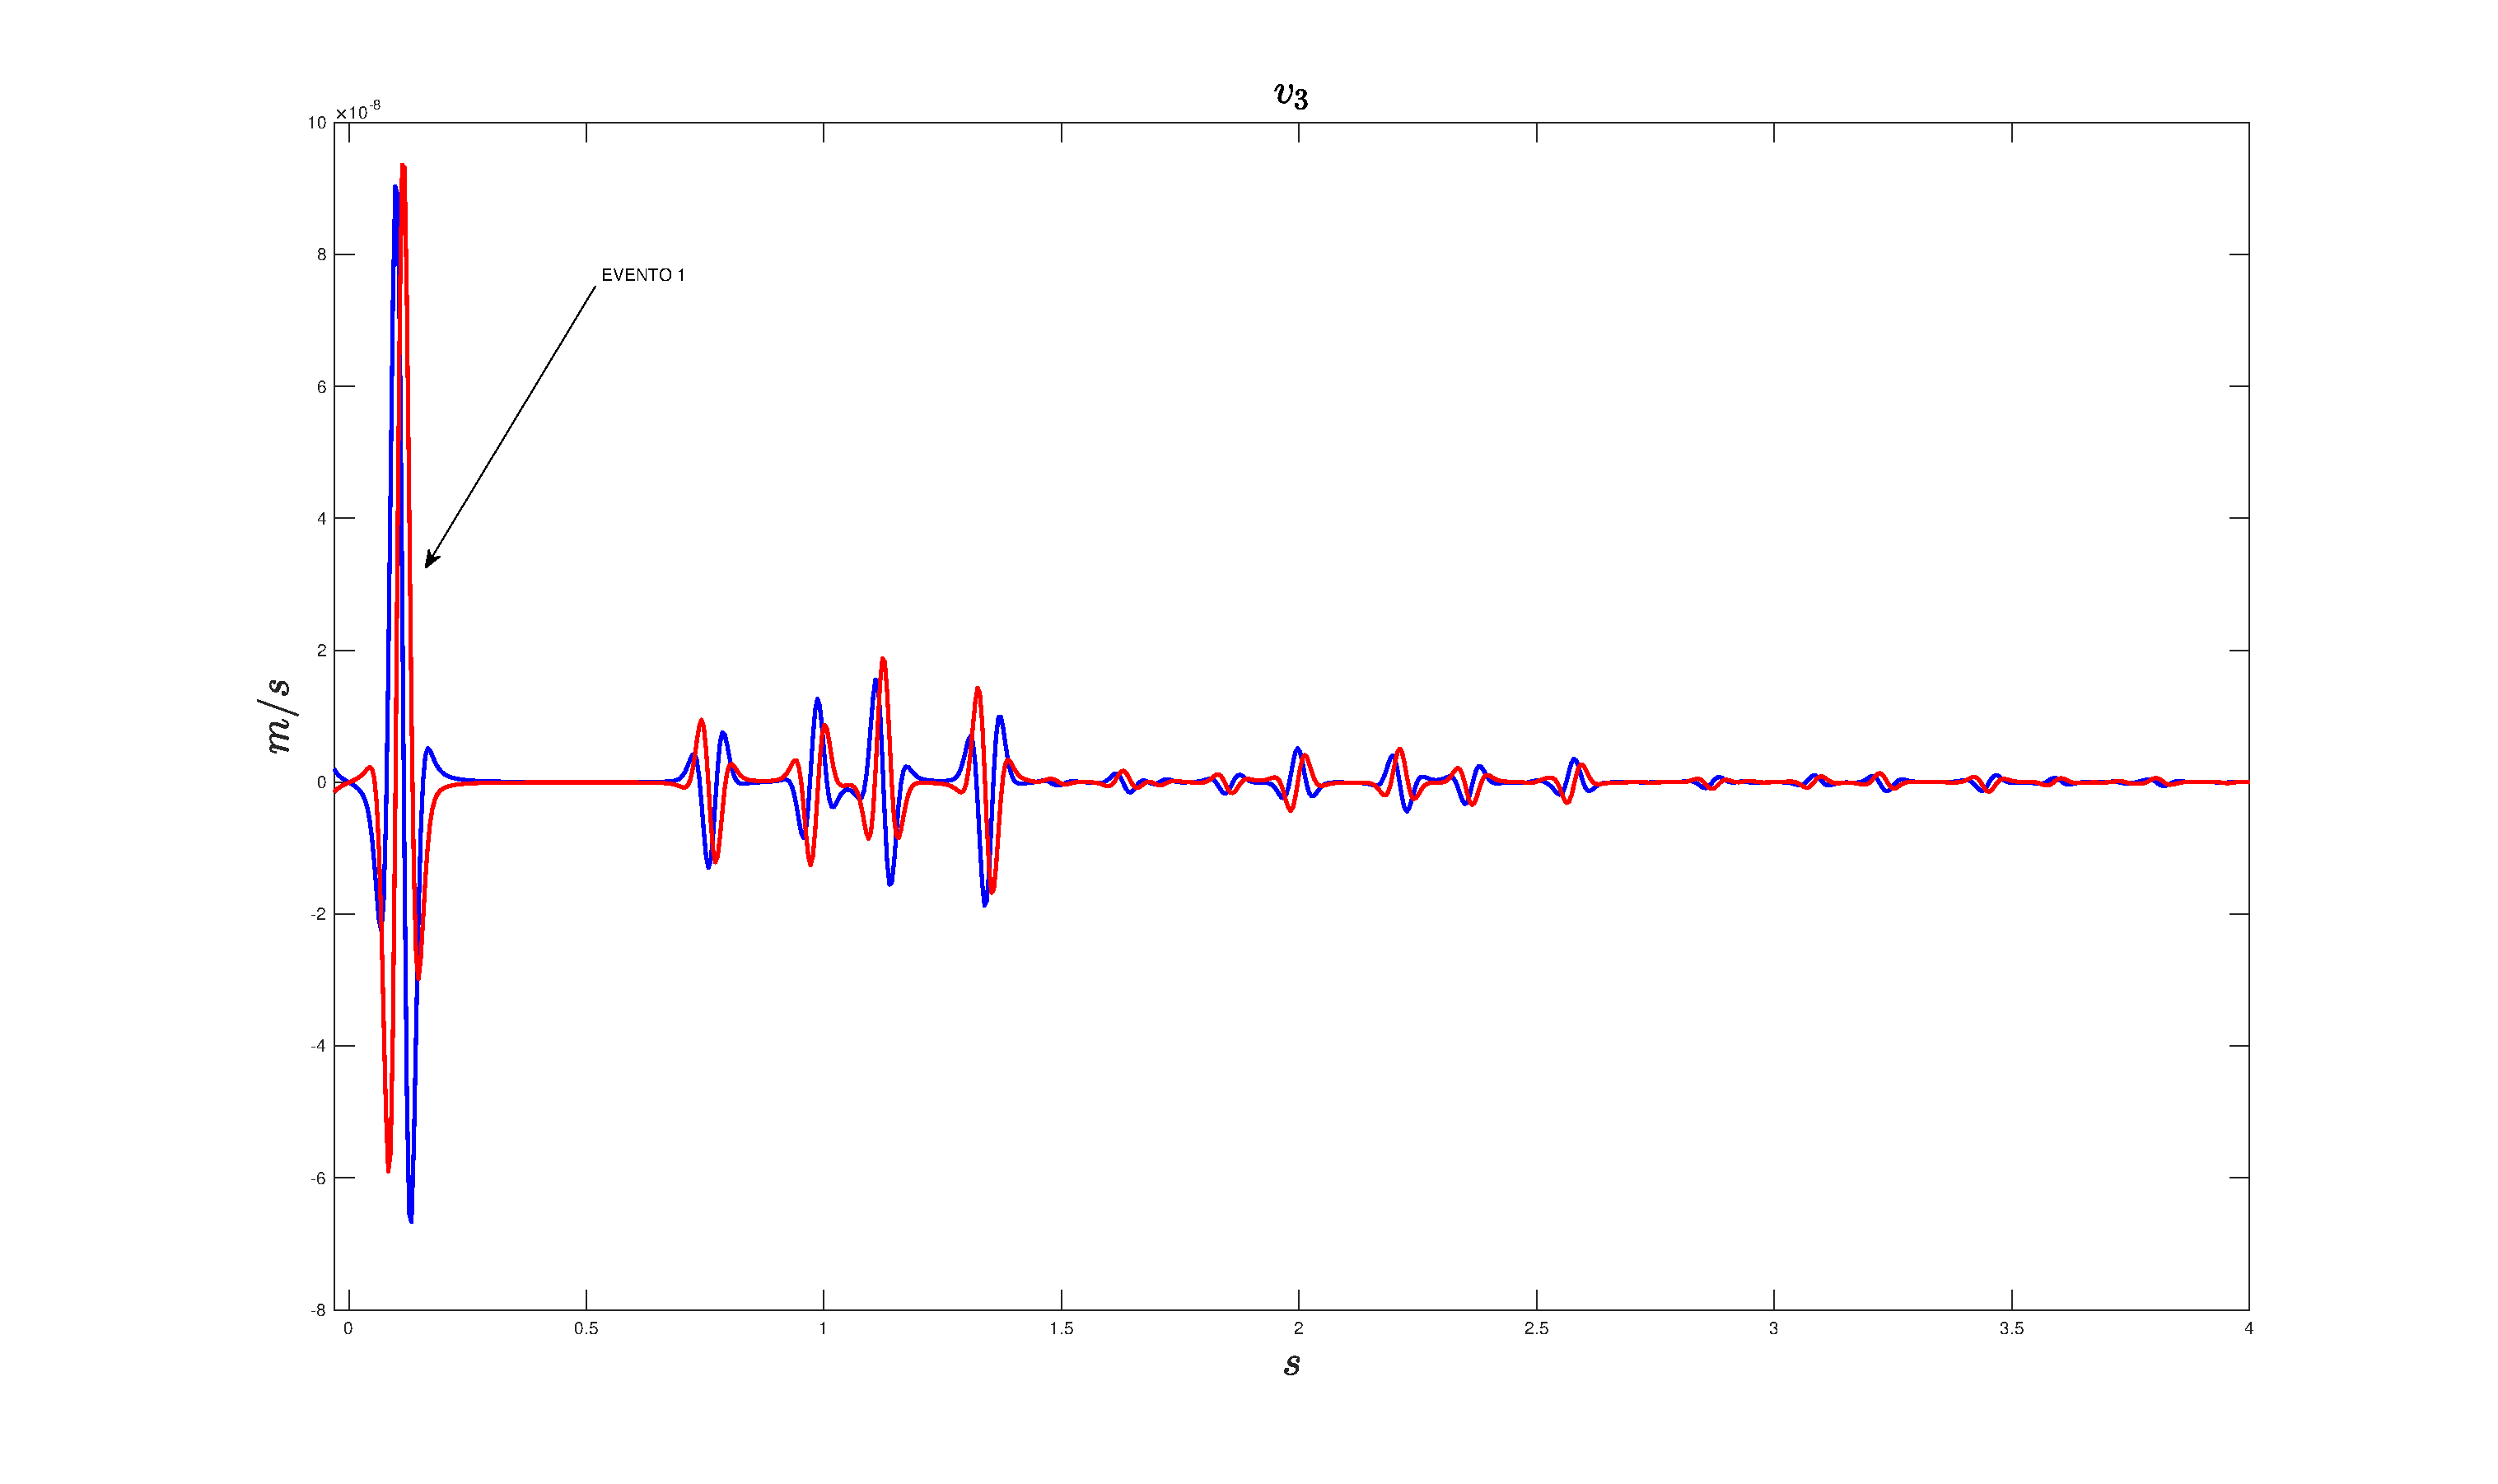
\includegraphics[scale=.678]{v3_250}\\
\caption{\textit{Modelo tridimensional, primeira camada com 1000 $m$, segunda camada com 500 $m$, fonte na superf\'icie e o receptor a 250 $m$ de profundidade verticalmente abaixo da fonte.}}
\label{fig.v3_250}
\end{figure}

Podemos observar, na figura (\ref{fig.v3}) que a amplitude da onda direta (evento 1) n\~ao est\'a satisfat\'oria como em casos anteriores. Nessa abordagem para o caso tridimensional temos uma quantidade maior de coeficientes e o algebrismo se torna menos trabalhoso se usarmos a velocidade de deslocamento do meio do que o pr\'oprio deslocamento do meio, pois economizamos a manipula\c{c}\~ao de alguns coeficientes. Talvez o algoritmo tenha dificuldade em identificar a velocidade de deslocamento do meio para onda direta quando fonte e receptor est\~ao na mesma posi\c{c}\~ao. Assim, afastamos o receptor da fonte, colocando-o numa profundidade vertical de $250\,m$, similar ao que fizemos anteriormente, e foi poss\'ivel identificar normalmente e chagada da onda direta. Na figura (\ref{fig.v3_250}), temos a chegada da onda direta (evento 1) para o mesmo modelo da figura (\ref{fig.v3}), com a \'unica diferen\c{c}a na dist\^ancia fonte/receptor. Note que o tempo de chegada da onda direta da figura (\ref{fig.v3_250}) coincide com o tempo de chegada da mesma onda na figura (\ref{fig.four_partially_1D_mech_hi_ampl_250}), pois em ambos os casos temos a mesma dist\^ancia fonte/receptor.\\











































